\documentclass[conference]{IEEEtran}
\IEEEoverridecommandlockouts
% The preceding line is only needed to identify funding in the first footnote. If that is unneeded, please comment it out.
\usepackage{cite}
\usepackage{amsmath,amssymb,amsfonts}
\usepackage{algorithmic}
\usepackage{graphicx}
\usepackage{textcomp}
\usepackage{xcolor}
\usepackage{tabularx}
\usepackage{multirow}
\usepackage{graphics} % for pdf, bitmapped graphics files
\usepackage{subfig}
\usepackage{subcaption}
\usepackage{hyperref}
\usepackage{academicons}
\usepackage{xcolor}
\usepackage{listings}
\def\BibTeX{{\rm B\kern-.05em{\sc i\kern-.025em b}\kern-.08em
		T\kern-.1667em\lower.7ex\hbox{E}\kern-.125emX}}
% Gráficas en MATLAB
\usepackage{tikz, pgfplots}
% Color Enlace
\definecolor{colorEnlace}{RGB}{0, 0, 0}
\hypersetup{
	colorlinks=true,
	linkcolor=colorEnlace,
	citecolor=colorEnlace,
	urlcolor=colorEnlace,
	pdfauthor={Davis Bremdow Salazar Roa},
	pdftitle={Introducción a LaTeX}
}
% Control 
\usepackage{amsmath}
\begin{document}
	
	\title{Experiencia N°3 - Identificación de Parámetros}
	% Ing. Diego Darcy Arredondo Huarac
	\author{	
		\IEEEauthorblockN{Davis Bremdow Salazar Roa}
		\IEEEauthorblockA{Universidad Nacional de San Antonio Abad del Cusco}
		\textit{Escuela Profesional de Ingeniería Electrónica}\\
		\textit{Laboratorio de Control I}\\
		200353 \\\\
		Cusco, Perú
	}
	
	\maketitle
	
	\begin{abstract}
		The mathematical modeling of a DC motor is based on differential equations that describe the dynamic relationship between the applied voltage, the current flowing through the motor winding, the torque, and the angular velocity generated. The model encompasses both electrical aspects, such as the rotor circuit's resistance and inductance, and mechanical aspects, including inertia and friction. These equations enable the prediction of motor performance in response to various inputs and operating conditions, aiding in the control of parameters in automation and robotics systems.
	\end{abstract}
	
	\begin{IEEEkeywords}
		Identificación de Parámetros, Toolbox MATLAB, Identificación del modelo de una planta, Sistemas electromecánicos
	\end{IEEEkeywords}
	
	\section{Introducción}
		El análisis del modelo matemático de un motor de corriente continua (DC) se basa en la representación de su comportamiento dinámico mediante ecuaciones diferenciales que describen la relación entre la tensión aplicada, la corriente que circula por el devanado del motor, y el par y la velocidad angular generados. Este modelo suele incluir tanto los aspectos eléctricos, como la resistencia y la inductancia del circuito del rotor, así como los aspectos mecánicos, como el momento de inercia y la fricción. Estas ecuaciones permiten predecir el rendimiento del motor en respuesta a diferentes entradas y condiciones de operación, facilitando el control de uno o varios parámetros en los sistemas de automatización y robótica.
	\section{Objetivos}
	
	\begin{itemize}
		\item Identificar el modelo de una planta.
		\item Analizar la respuesta en el tiempo del modulo hallado.
	\end{itemize}
	
	\section{Hallar el modelo matemático del motor DC, considerando la $\omega (S)$ como la salida y $E_a(S)$ como la entrada}
	
	Un motor de corriente continua (DC) representa un sistema híbrido que aúna los fenómenos eléctricos y mecánicos en un sistema que rescatar las mejores características de cada uno con la finalidad de poder crear sistemas capaces de control de posición y/o transporte.
	
	Para el análisis del sistema electromecánico (motor DC) propuesto en la figura \ref{fig:motor-electromecanico} se sub-dividio el mismo en 2 partes (eléctrica y mecánica) y en las cuales se aplicaran los diferentes teoremas que relacionan sus diferentes parámetros siendo el caso por ejemplo para el sistema eléctrico el uso de la ley de Tensiones de Kirchhoff y en el caso mecánico el empleo de los diagramas de cuerpo libre que nos permitirán analizar y relacionar todas las fuerzas que interactúan en el sistema.
	
	\begin{figure}[h]
		\centering
		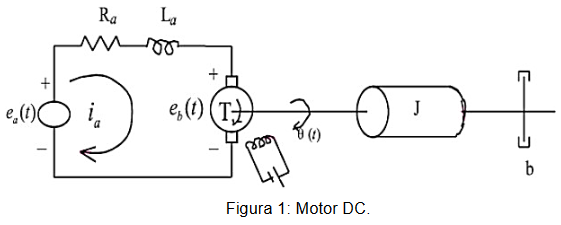
\includegraphics[width=0.4\textwidth]{media/motor-electromecanico}
		\caption{Esquema general de un motor DC}
		\label{fig:motor-electromecanico}
	\end{figure}
	
	Al aplicar la ley de tensiones de Kircchoff en el circuito de armadura, se tiene la siguiente relación:
	\begin{equation}
		R_ai(t) + L\frac{d}{dx} i(t) + K_b \frac{d}{dt} \theta (t) = e_a(t)
		\label{eq:malla-1}
	\end{equation}
	
	Esta relación eléctrica nos permite relacionar voltajes entre los diferentes componentes que integran al circuito de armadura del motor y la cual a su vez describen la parte eléctrica del sistema, siendo tales partes las siguientes y las que se considerarán para el modelo a construir en MATLAB. \\
	
	$R_a = 17 \Omega$ \\
	$L_a = 9.35*10^{-3} H$ \\
	$K_e = 0.0436 \frac{Vs}{rad}$ \\
	$K_m = 0.0436 \frac{N-m}{A}$ \\
	
	Además en la ecuación \ref{eq:malla-1} se debe tener en cuenta la equivalencia para la constante contra electromotriz y la cual esta relacionada con la frecuencia angular mediante la siguiente expresión
	\begin{equation}
		e_b(t) = K_e\frac{d}{dt} \theta(t)
		\label{eq:contra-electromotriz}
	\end{equation}
	
	Obteniéndose de esta forma la ecuación \ref{eq:malla-1}, al analizar tal expresión se puede destacar que se cuenta con un termino en función de la frecuencia angular, sin embargo aun es necesario despejar la corriente en función del anterior parámetro, por ello es necesario utilizar la siguiente constante (par del motor) $K_m$ y los diagramas de cuerpo libre en la parte mecánica, obteniéndose las siguientes relaciones:
	
	\begin{align}
		T &= \ddot{\theta}J + \dot{\theta}b \label{eq:diagrama-cuerpo-libre}\\ 
		T &= K_mi(t) \label{eq:constate-torque}
	\end{align}
	
	Al reemplazar la ecuación \ref{eq:diagrama-cuerpo-libre} y \ref{eq:constate-torque} y despejar la corriente, se tiene la siguiente expresión analítica:
	
	\begin{equation}
		i(t) = \frac{ \ddot{\theta}J + \dot{\theta}b }{ K_m }
		\label{eq:corriente-torque}
	\end{equation}
	
	Una vez obtenidas todas estas relaciones será necesario aplicar la transformada de Laplace $\mathcal{L}\{f(t)\}$ para transformar cada ecuación al dominio de la frecuencia y obtener una relación entre la $\omega(s)$ (frecuencia angular) y $E_a(S)$ la cual es la función de transferencia deseada, obteniendo.
	
	\begin{align}
		E_a(S) &= I(S)\{R_a + LS\} + K_eS\theta(S) \label{eq:malla-1-laplace} \\
		T(S) &= \theta(S)JS^2 + \theta(S)bS \label{eq:torque-laplace} \\
		I(S) &= \frac{\theta(S)JS^2 + \theta(S)bS}{K_m} \label{eq:corriente-laplace}
	\end{align}
	
	Finalmente al reemplazar la ecuación \ref{eq:corriente-laplace} en \ref{eq:malla-1-laplace} se tendrá la siguiente expresión resultante de la cual será posible obtener la función de transferencia, la cual se representa de la siguiente forma:
	
	\begin{equation}
		\frac{\omega(S)}{E_a(S)} = \frac{K_m}{JLS^2 + (JR_a + Lb)S + (bR_a + K_eK_m)}
		\label{eq:ft-motor}
	\end{equation}
	
	De esta expresión final además se tiene que considerar la influencia de la parte mecánica en las cuales esta involucrada la inercia y el coeficiente de fricción viscosa perteneciente al amortiguador, considerando para ello. \\
	
	$J = 1.6*10^{-6} kg-m^2$ \\
	$b = 1.4*10^{-6} \frac{N -m}{s-rad}$
	
	Al reemplazar los valores numéricos en la expresión literal de la ecuación \ref{eq:ft-motor}, se tiene:
	
	\begin{equation}
		\frac{\omega(S)}{E_a(S)} = \frac{0.0436}{1.496*10^{-8}S^2 + 2.721*10^{-5}S + 0.001925}
		\label{eq:ft-motor-literal}
	\end{equation}
	
	\section{Usando el sotfware MATLAB simule el modelo del motor cuando la entrada es un escalón}
	
	Al considerar la función de transferencia final obtenida en \ref{eq:ft-motor-literal} y al aplicar una escalón unitario se obtiene la siguiente respuesta 
	
	\begin{figure}[h]
		\centering
		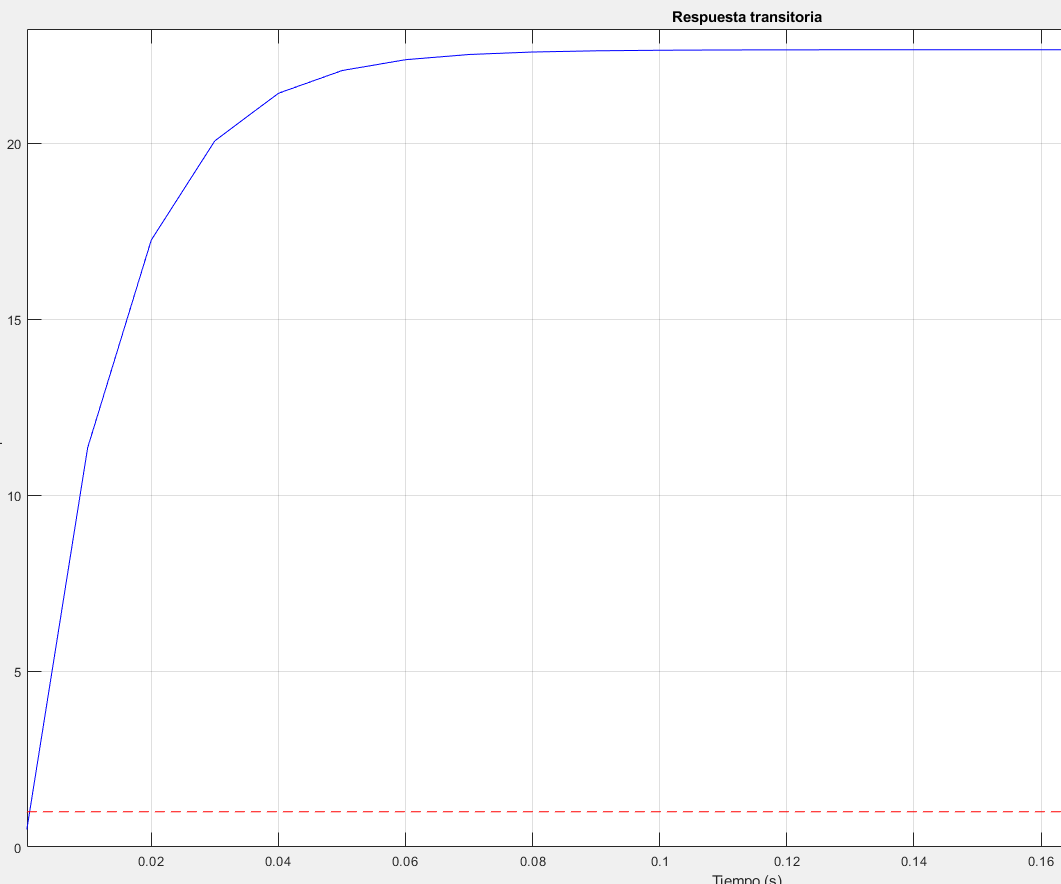
\includegraphics[width=0.4\textwidth]{media/resp-escalon}
		\caption{Respuesta del sistema frente al escalón unitario}
		\label{fig:resp-escalon}
	\end{figure}
	
	De la figura \ref{fig:resp-escalon} se puede determinar que el sistema es de rápida respuesta y que cuenta con una ganancia que eleva la salida hasta un valor de máximo equivalente a 22.65[V], además este al ser un sistema de 2do como se define en \cite{ogata2015} se puede analizar los parámetros para obtener una respuesta más comprensible sobre el funcionamiento del sistema.
	
	Para poder analizar el tiempo de respuesta del sistema y el tipo de sistema se dividió a cada termino del mismo por el coeficiente del termino cuadrático obtenido la siguiente expresión
	\begin{equation}
		\frac{\omega(S)}{E_a(S)} = \frac{K*128660.43}{S^2 + 1819.0568S + 128660.43}
		\label{eq:ft-motor-reducida}
	\end{equation}
	
	Y de la cual se podrá obtener la valor de K o ganancia, $\xi$, frecuencia natural $\omega_n$ y el tiempo de establecimiento del sistema $T_e$ en función a la constante de tiempo $\tau$, al realizar las operaciones para cada caso se obtuvieron los siguientes datos. \\
	
	
	$K = 22.65$ \\
	$\omega_n = 358.69 \frac{rad}{s}$ \\
	$\xi = 2.5367$ \\
	$\tau = 0.01413 [s]$ \\
	$T_e (2\%)= 0.0565  [s]$ \\
	
	Parámetros de los cuales se puede inferir que el sistema a analizar será uno sobre amortiguado debido al valor de al valor de $\xi$ mayor 1 y con una ganancia diferente a 1 y una rápida respuesta frente a una entrada y un tiempo de establecimiento al 2\%.
	
	Para la obtención de todos estos parámetros fue necesario hacer uso de la herramienta de programación MATLAB y cuyo código se detalla de la siguiente forma:
	
	\lstset{
		language=Matlab, % Define el lenguaje
		basicstyle=\ttfamily\small, % Tamaño de letra pequeño
		keywordstyle=\color{blue}, % Color de las palabras clave
		commentstyle=\color{green}, % Color de los comentarios
		stringstyle=\color{red}, % Color de las cadenas de texto
		numbers=left, % Muestra los números de línea a la izquierda
		numberstyle=\tiny\color{gray}, % Estilo de los números de línea
		stepnumber=1, % Muestra un número en cada línea
		breaklines=true, % Ajuste automático de línea
		frame=single, % Borde alrededor del código
		xleftmargin=0em, % Elimina el margen izquierdo
		framexleftmargin=0em % Elimina el espacio dentro del marco izquierdo
	}
	
	\begin{lstlisting}
		Kt = 0.0436;
		Kb = 0.0436;
		Ra = 17;
		L = 9.35e-3;
		J = 1.6e-6;
		b = 1.4e-6;
		
		numerador = [Kt];
		denominador = [J*L (J*Ra + L*b) (b*Ra + Kb*Kt)];
		
		H = tf(numerador, denominador)
		
		t = linspace(0,10,10000);    
		u = ones(size(t));
		
		y1 = lsim(H,u,t);
		figure;
		plot(t,y1,'b',t,u,'r--')
		xlabel('Tiempo (s)')
		ylabel('Amplitud')
		title('Respuesta transitoria')
		grid on
	\end{lstlisting}
	
	\section{Describa en que consiste el toolbox de identificación de sistemas de Matlab}
	
	El toolbox de identificación de sistemas de MATLAB permite construir modelos matemáticos que describen sistemas dinámicos a partir de datos experimentales el cual consta de varias herramientas y procedimientos para la obtención y caracterización de parámetros de un sistema, teniendo a grandes rasgos los siguientes pasos:
	\begin{itemize}
		\item Importación de datos
		\item Preprocesamiento de los datos
		\item Selección del tipo de modelo
		\item Estimación de los parámetros del modelo
		\item Validación del modelo
		\item Ajuste y refinamiento del modelo
		\item Uso del modelo
		\item Análisis y exportación del modelo
	\end{itemize}
	
	\subsection{Importación de datos}
	El primer paso consiste en importar los datos del sistema que incluyen las señales de entrada, salida y el tiempo de muestreo, esto se puede hacer mediante el siguiente código de programación en MATLAB
	
	\begin{lstlisting}
		data = iddata(salida, entrada, Ts);
	\end{lstlisting}
	
	\subsection{Preprocesamiento de los datos}
	Antes de realizar la identificación, es fundamental preprocesar los datos para mejorar la precisión del modelo. Esto incluye eliminar tendencias y dividir los datos en subconjuntos de entrenamiento y validación, para ello se puede usar como ejemplo
	
	\begin{lstlisting}
		data_pre = detrend(data);  % Eliminar tendencia
		[train_data, val_data] = split(data_pre, 0.7);  % Dividir los datos
		
	\end{lstlisting}
	
	\subsection{Selección del tipo de modelo}
	Dependiendo del sistema, se puede seleccionar un modelo paramétrico (ARX, ARMAX, OE, etc.) o no paramétrico. La selección del modelo es clave para una buena identificación, este paso es relevante debido a que determina la naturaleza del sistema que se desea analizar, por lo tanto en tal modelo será necesario que se desea obtener una función de transferencia, un ejemplo de esto puede ser lo siguiente 
	\begin{lstlisting}
		model_arx = arx(train_data, [na nb nk])
	\end{lstlisting}
	
	Los siguientes pasos a realizar solo son parte del post procesado de información, para ajustar el modelo en caso se requiera mayor precisión para ello.
	
	\subsection{Estimación de los parámetros del modelo}
	Después de seleccionar el tipo de modelo, se deben estimar los parámetros que mejor se ajusten a los datos de entrenamiento.
	
	\subsection{Validación del modelo}
	Es importante validar el modelo utilizando datos de validación para asegurarse de que el modelo sea representativo del sistema real.
	
	\subsection{Ajuste y refinamiento del modelo}
	Si el modelo no es suficientemente preciso, se pueden refinar los parámetros o probar con otro tipo de modelo.
	
	\subsection{Uso del modelo}
	Una vez validado, el modelo puede utilizarse para simulaciones, predicciones o diseño de controladores.
	
	\subsection{Análisis y exportación del modelo}
	Finalmente, se puede analizar el comportamiento del modelo (por ejemplo, mediante diagramas de Bode) y exportarlo para su uso posterior.
	
	\section{Conclusiones}
	
	El modelo matemático obtenido para el motor DC permite identificar claramente la relación entre la entrada de voltaje y la velocidad angular del sistema, lo que facilita su análisis y control en aplicaciones de automatización y robótica.
	
	La simulación realizada en MATLAB confirma que el sistema tiene una respuesta rápida con características de sobreamortiguamiento, lo que lo hace adecuado para aplicaciones donde se requiere un control preciso y estable del motor.
	
	\bibliographystyle{IEEEtran}
	\bibliography{biblio}
\end{document}
